\chapter{Quick Revision: OE-EC803A - Internet of Things (IoT)}

This high-density revision sheet compiles core definitions, mathematical formulas, essential diagrams to practice drawing, frequently asked short questions, and fast-recall points across all 10 units of the syllabus.


\section{Important Definitions}

\subsection{Unit I: Introduction}
\begin{itemize}
  \item   \textbf{Internet of Things (IoT):} A network of physical objects ("things") embedded with sensors, software, and technologies to connect and exchange data with other devices and systems over the internet.
  \item   \textbf{Enchanted Objects:} Everyday physical items (e.g., pens, umbrellas, tables) enhanced with internet connectivity, computation, and subtle interfaces to make them more useful without being intrusive.
  \item   \textbf{Ubiquitous Computing:} A paradigm where computing is made to appear anytime and everywhere, integrated seamlessly into everyday objects and environments.
\end{itemize}

\subsection{Unit II: Design Principles}
\begin{itemize}
  \item   \textbf{Calm Technology:} Technology that informs the user but does not demand their primary attention; it moves back and forth between the periphery and center of attention.
  \item   \textbf{Ambient Device:} A physical object designed to display information (e.g., changes in weather or stock markets) in a subtle, non-intrusive way through light, color, or movement.
  \item   \textbf{Magic as Metaphor:} Using magic-like interactions (e.g., waving a hand to turn on a lamp) as user interface models to mask underlying complex technologies.
  \item   \textbf{Affordance:} The physical properties of an object that suggest how it should be used (e.g., a button invites pushing, a knob invites turning).
\end{itemize}

\subsection{Unit III: Internet Principles}
\begin{itemize}
  \item   \textbf{TCP/IP Suite:} The conceptual model and set of communications protocols used on the internet, organized into 4 layers (Application, Transport, Internet, Network Access).
  \item   \textbf{UDP (User Datagram Protocol):} A lightweight, connectionless transport protocol that prioritizes speed and low latency over reliability.
  \item   \textbf{DHCP (Dynamic Host Configuration Protocol):} An application layer protocol that automates the assignment of IP addresses, gateways, and DNS settings.
  \item   \textbf{DNS (Domain Name System):} The hierarchical system that translates human-readable domain names (e.g., `iot.org`) into numeric IP addresses.
  \item   \textbf{MAC Address:} A unique 48-bit physical hardware identifier burned into a network interface controller (NIC) by the manufacturer.
\end{itemize}

\subsection{Unit IV: Prototyping}
\begin{itemize}
  \item   \textbf{Sketching:} Rapid, low-cost, and low-fidelity physical or digital drawing used to visualize and iterate concepts during early design phases.
  \item   \textbf{Open-Source Hardware:} Physical electronics platforms (e.g., Arduino, ESP32) whose design schematics, PCB layouts, and source codes are publicly available for modification.
\end{itemize}

\subsection{Unit V: Prototyping Physical Design}
\begin{itemize}
  \item   \textbf{Additive Manufacturing (3D Printing):} Enclosure production by melting and depositing material (e.g., plastic filament in FDM) layer-by-layer from a 3D digital model.
  \item   \textbf{Subtractive Manufacturing:} Creating parts by removing material from a solid sheet or block (e.g., Laser Cutting for 2D profiles, CNC Milling for 3D blocks).
  \item   \textbf{Repurposing:} Modifying pre-existing, off-the-shelf enclosures to house prototype electronics.
\end{itemize}

\subsection{Unit VI: Prototyping Embedded Devices}
\begin{itemize}
  \item   \textbf{Microcontroller (MCU):} A single integrated circuit containing a processor core, memory (RAM/Flash), and programmable input/output peripherals (e.g., ATMega328).
  \item   \textbf{Microprocessor (MPU):} A general-purpose processor (e.g., Broadcom ARM on Raspberry Pi) that requires external RAM, Flash, and an operating system to function.
  \item   \textbf{I2C (Inter-Integrated Circuit):} A synchronous, multi-master, multi-slave, half-duplex 2-wire serial bus (SDA, SCL).
  \item   \textbf{SPI (Serial Peripheral Interface):} A synchronous, 4-wire, full-duplex serial bus (MOSI, MISO, SCK, CS).
  \item   \textbf{UART (Universal Asynchronous Receiver-Transmitter):} An asynchronous, 2-wire, point-to-point communication protocol (TX, RX).
  \item   \textbf{BlinkUp (Electric Imp):} A proprietary optical method that uses a smartphone screen flash to transmit Wi-Fi SSID and credentials to an IoT photodiode sensor.
\end{itemize}

\subsection{Unit VII: Prototyping Online Components}
\begin{itemize}
  \item   \textbf{REST API:} A stateless, request-response web service architecture that maps operations to standard HTTP verbs (GET, POST, PUT, DELETE).
  \item   \textbf{WebSockets:} A protocol providing full-duplex, persistent, single-socket communication channels over a single TCP connection.
  \item   \textbf{MQTT Broker:} The central server in a publish/subscribe network that receives messages from publishers and routes them to subscribed clients.
\end{itemize}

\subsection{Unit VIII: Embedded Code Development \& Business Models}
\begin{itemize}
  \item   \textbf{Over-The-Air (OTA):} Wireless transmission and installation of firmware updates directly onto deployed IoT devices.
  \item   \textbf{Business Model Canvas:} A visual chart containing 9 building blocks (Value Propositions, Channels, etc.) used to describe, design, and pivot a startup's strategy.
  \item   \textbf{Lean Startup:} A methodology that favors experimentation, customer feedback, and iterative design (Build-Measure-Learn) over elaborate planning.
\end{itemize}

\subsection{Unit IX: Moving to Manufacture}
\begin{itemize}
  \item   \textbf{Gerber File:} The standard vector format file set containing instructions for PCB manufacturing (copper layers, solder mask, drill locations).
  \item   \textbf{AOI (Automated Optical Inspection):} Camera-based quality assurance that checks assembled boards for missing or misaligned components.
  \item   \textbf{In-Circuit Test (ICT):} Electrical probe verification checking for component value accuracy and trace shorts/opens on assembled PCBs.
  \item   \textbf{Burn-In Test:} Operating a device under maximum stress conditions (elevated temperature/voltage) for 24-72 hours to detect infant mortality failures.
\end{itemize}

\subsection{Unit X: Ethics}
\begin{itemize}
  \item   \textbf{Smart City:} An urban area integrating IoT sensors and ICT to optimize traffic, lighting, waste, and municipal resource management.
  \item   \textbf{Intelligent Transportation Systems (ITS):} IoT transport applications integrating V2X communication to track vehicles and optimize public transit schedules.
  \item   \textbf{Surveillance Creep:} The gradual expansion of continuous ambient monitoring into private and public spaces without clear user consent.
  \item   \textbf{Privacy by Design:} Building data minimization, encryption, and local edge processing into the product architecture from inception.
\end{itemize}


\section{Key Formulas}

\subsection{1. Wavelength \& Antenna Length}
The length ($L$) of a quarter-wave ($1/4\lambda$) wire antenna is calculated as:
\[ \lambda = \frac{c}{f} \]
\[ L = \frac{\lambda}{4} = \frac{c}{4f} \]

\begin{itemize}
  \item   Where:
  \item   $\lambda$ = Wavelength of the radio signal (meters, $\text{m}$)
  \item   $c$ = Speed of light in vacuum ($\approx 3 \times 10^8\text{ m/s}$)
  \item   $f$ = Transmitting frequency ($\text{Hz}$)
  \item   $L$ = Quarter-wave wire antenna length (meters, $\text{m}$)
\end{itemize}
\textit{   }Example (2.4 GHz Wi-Fi/BLE):*
    \[ L = \frac{3 \times 10^8\text{ m/s}}{4 \times (2.4 \times 10^9\text{ Hz})} \approx 0.03125\text{ m} \approx \mathbf{3.13\text{ cm}} \]

\subsection{2. IPv4 Host Capacity}
The number of available host IP addresses on an IPv4 subnet is:
\[ \text{Hosts} = 2^{32 - N} - 2 \]

\begin{itemize}
  \item   Where:
  \item   $N$ = CIDR subnet mask prefix length (e.g., $N = 24$ for $255.255.255.0$).
  \item   The subtraction of $2$ accounts for the reserved network address and the broadcast address.
\end{itemize}


\section{Diagrams to Practice Drawing}

Prepare to sketch these block architectures and flowcharts by hand for long-form answers:

\subsection{1. WWW vs. IoT Comparison (Unit I)}
Mappings of human-centric vs. machine-to-machine communications.  
\begin{figure}[H]
\centering
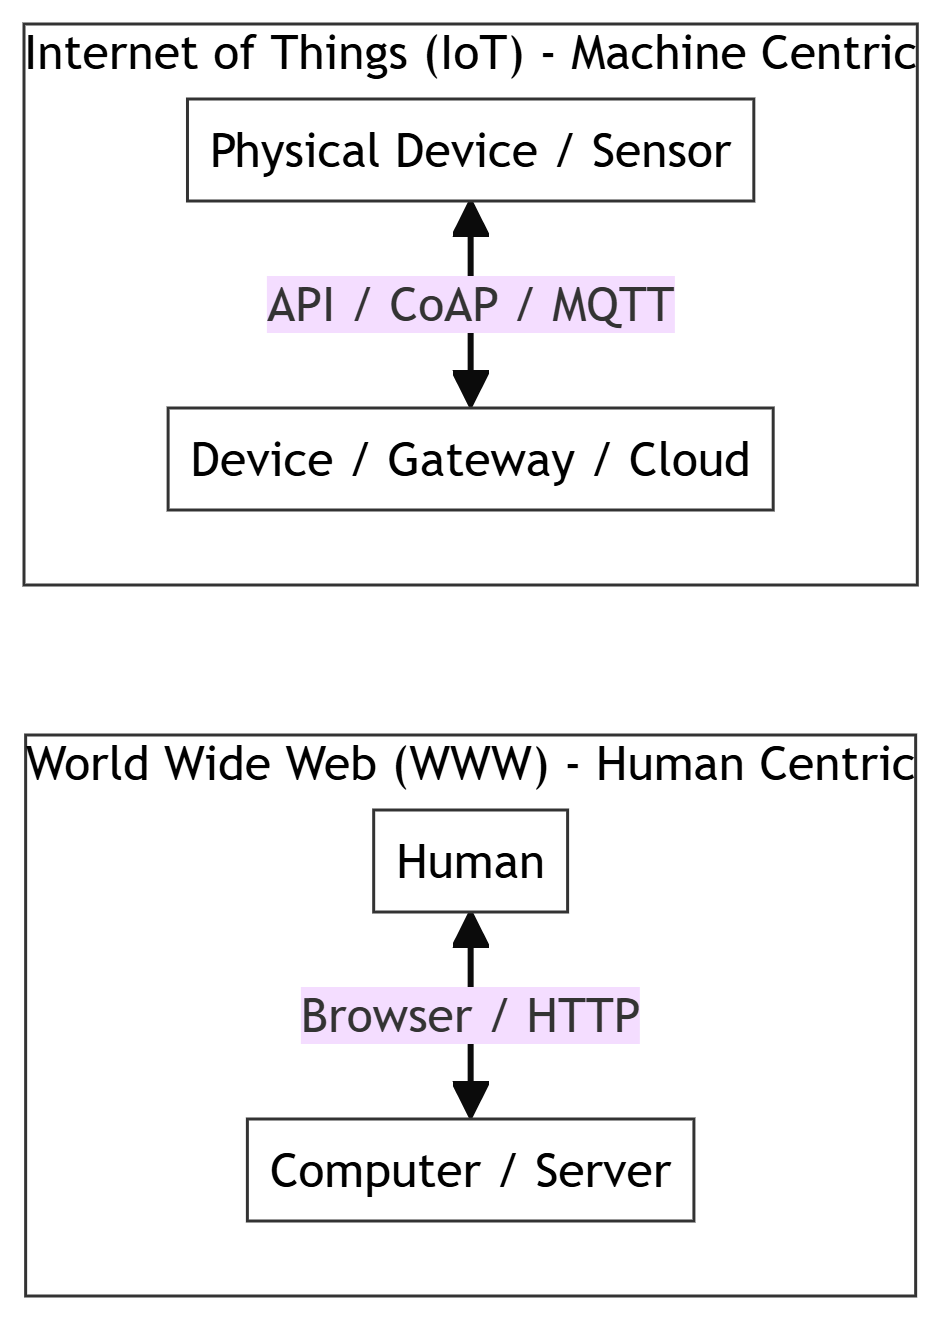
\includegraphics[width=0.75\textwidth,height=0.32\textheight,keepaspectratio]{../Images/chapter_01/www_vs_iot.png}
\caption{WWW vs. IoT Comparison}
\end{figure}

\subsection{2. ETSI M2M Functional Architecture (Unit I)}
Device, gateway, and network domain blocks.  
\begin{figure}[H]
\centering
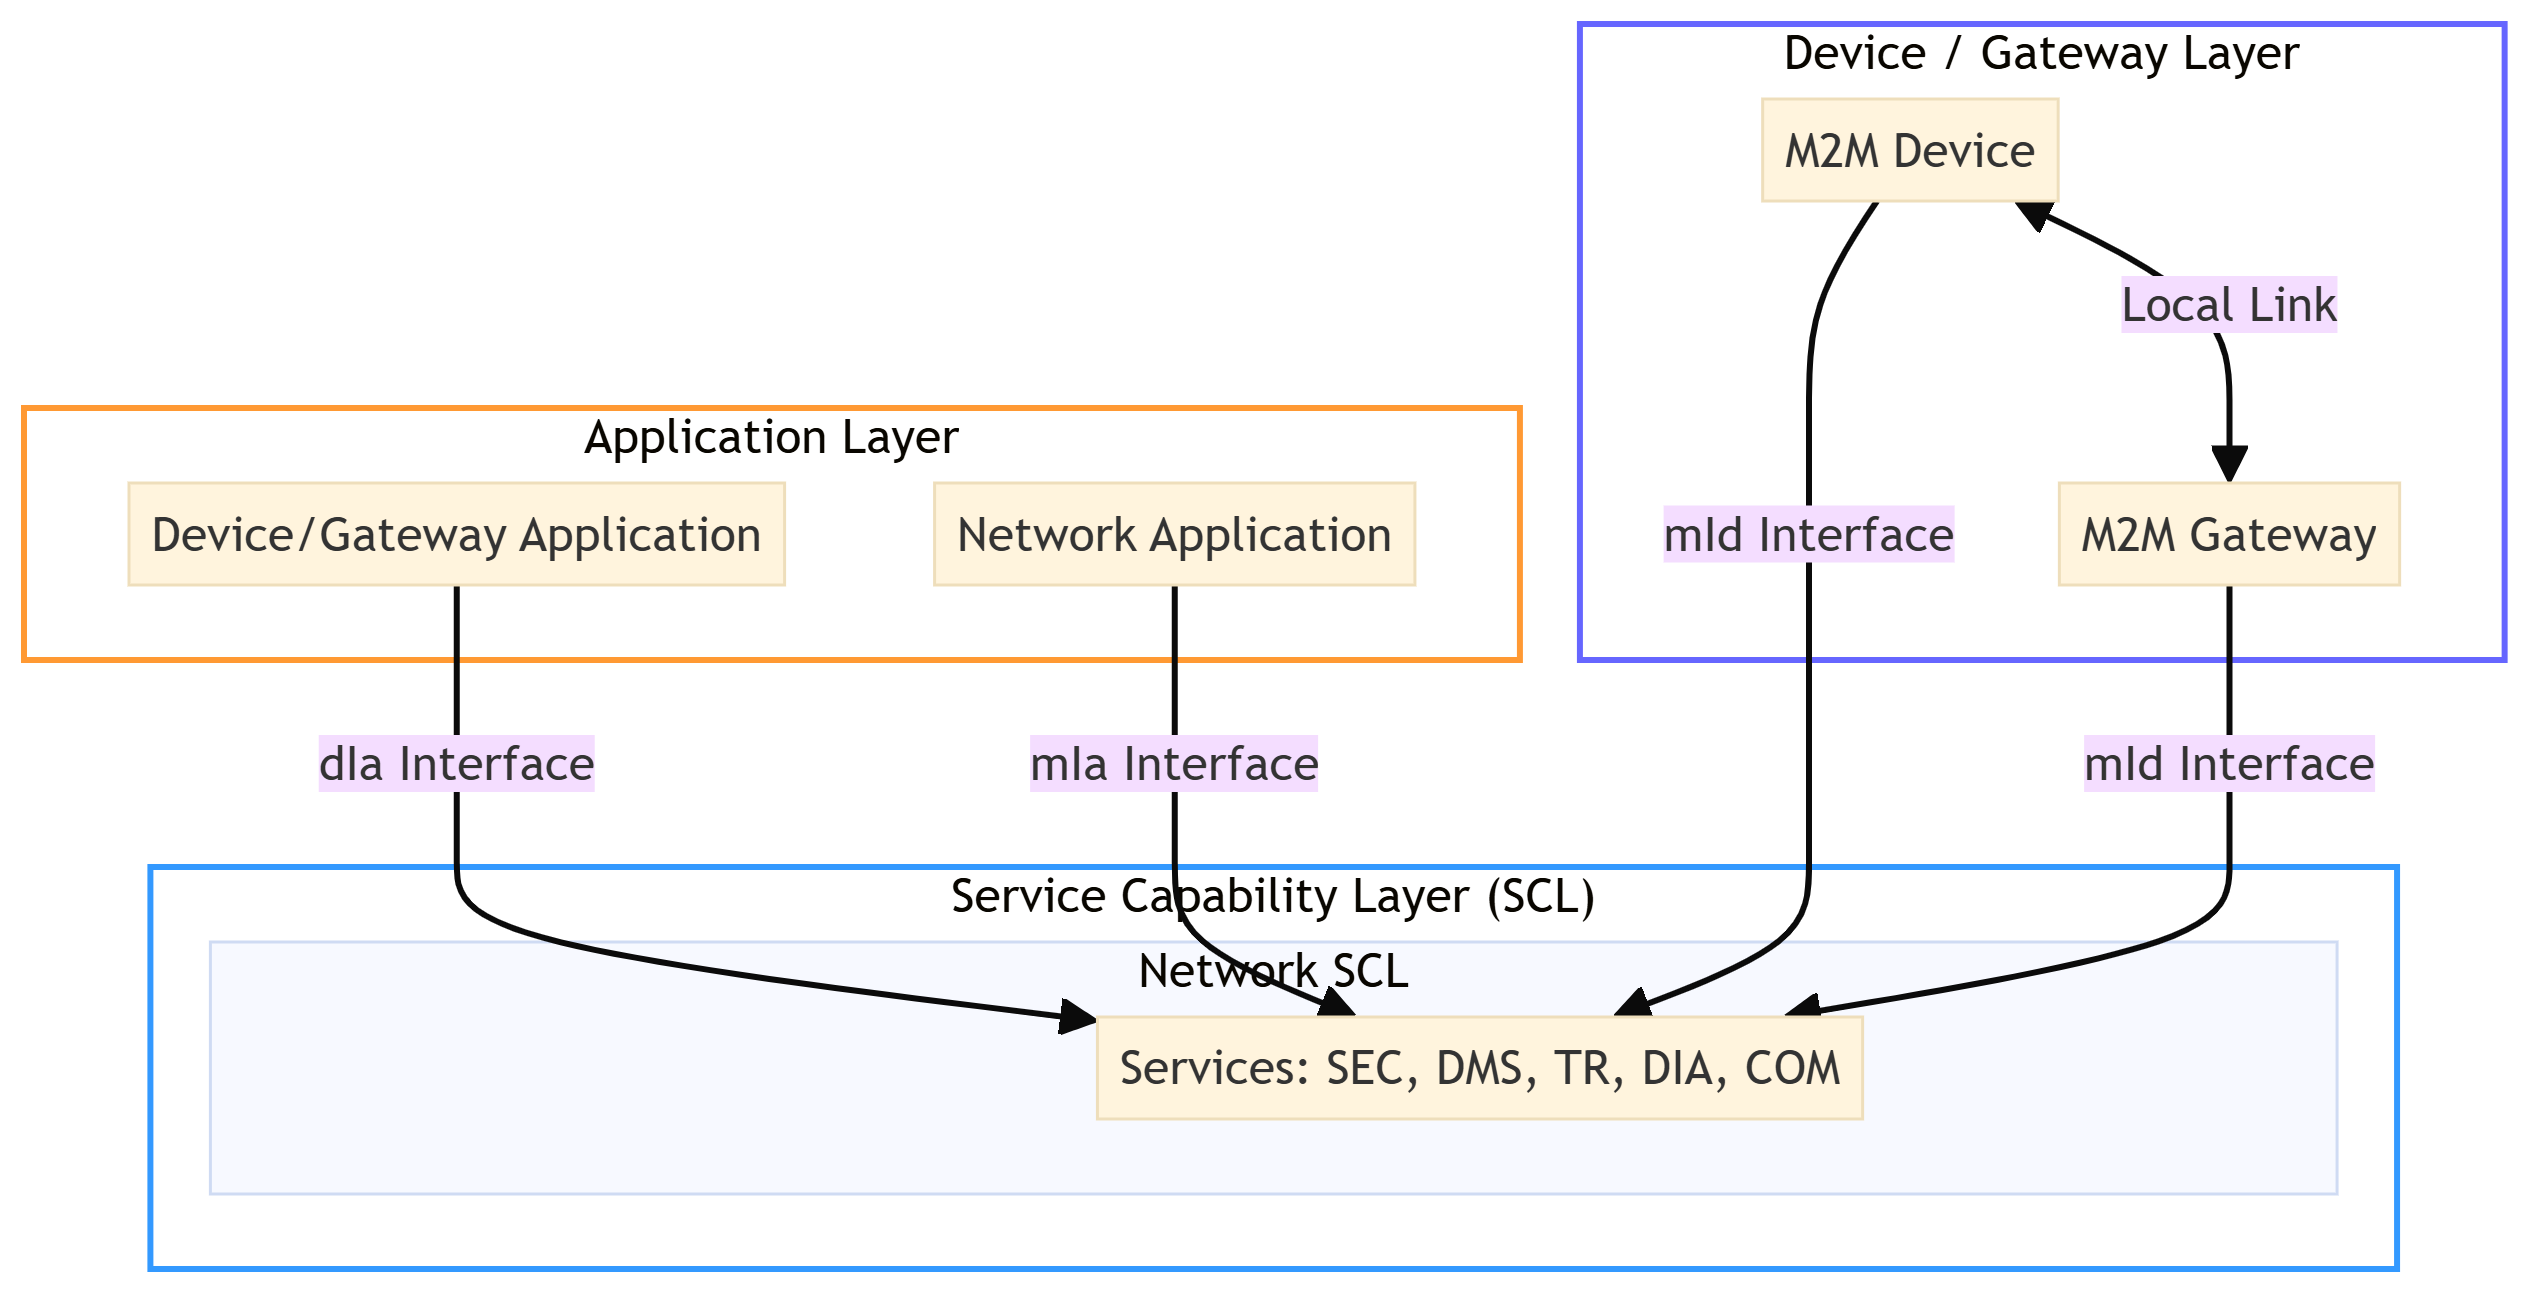
\includegraphics[width=0.75\textwidth,height=0.32\textheight,keepaspectratio]{../Images/chapter_01/etsi_m2m_architecture.png}
\caption{ETSI M2M Functional Architecture}
\end{figure}

\subsection{3. DHCP DORA Handshake (Unit III)}
Sequence flow of DISCOVER $\to$ OFFER $\to$ REQUEST $\to$ ACK.  
\begin{figure}[H]
\centering
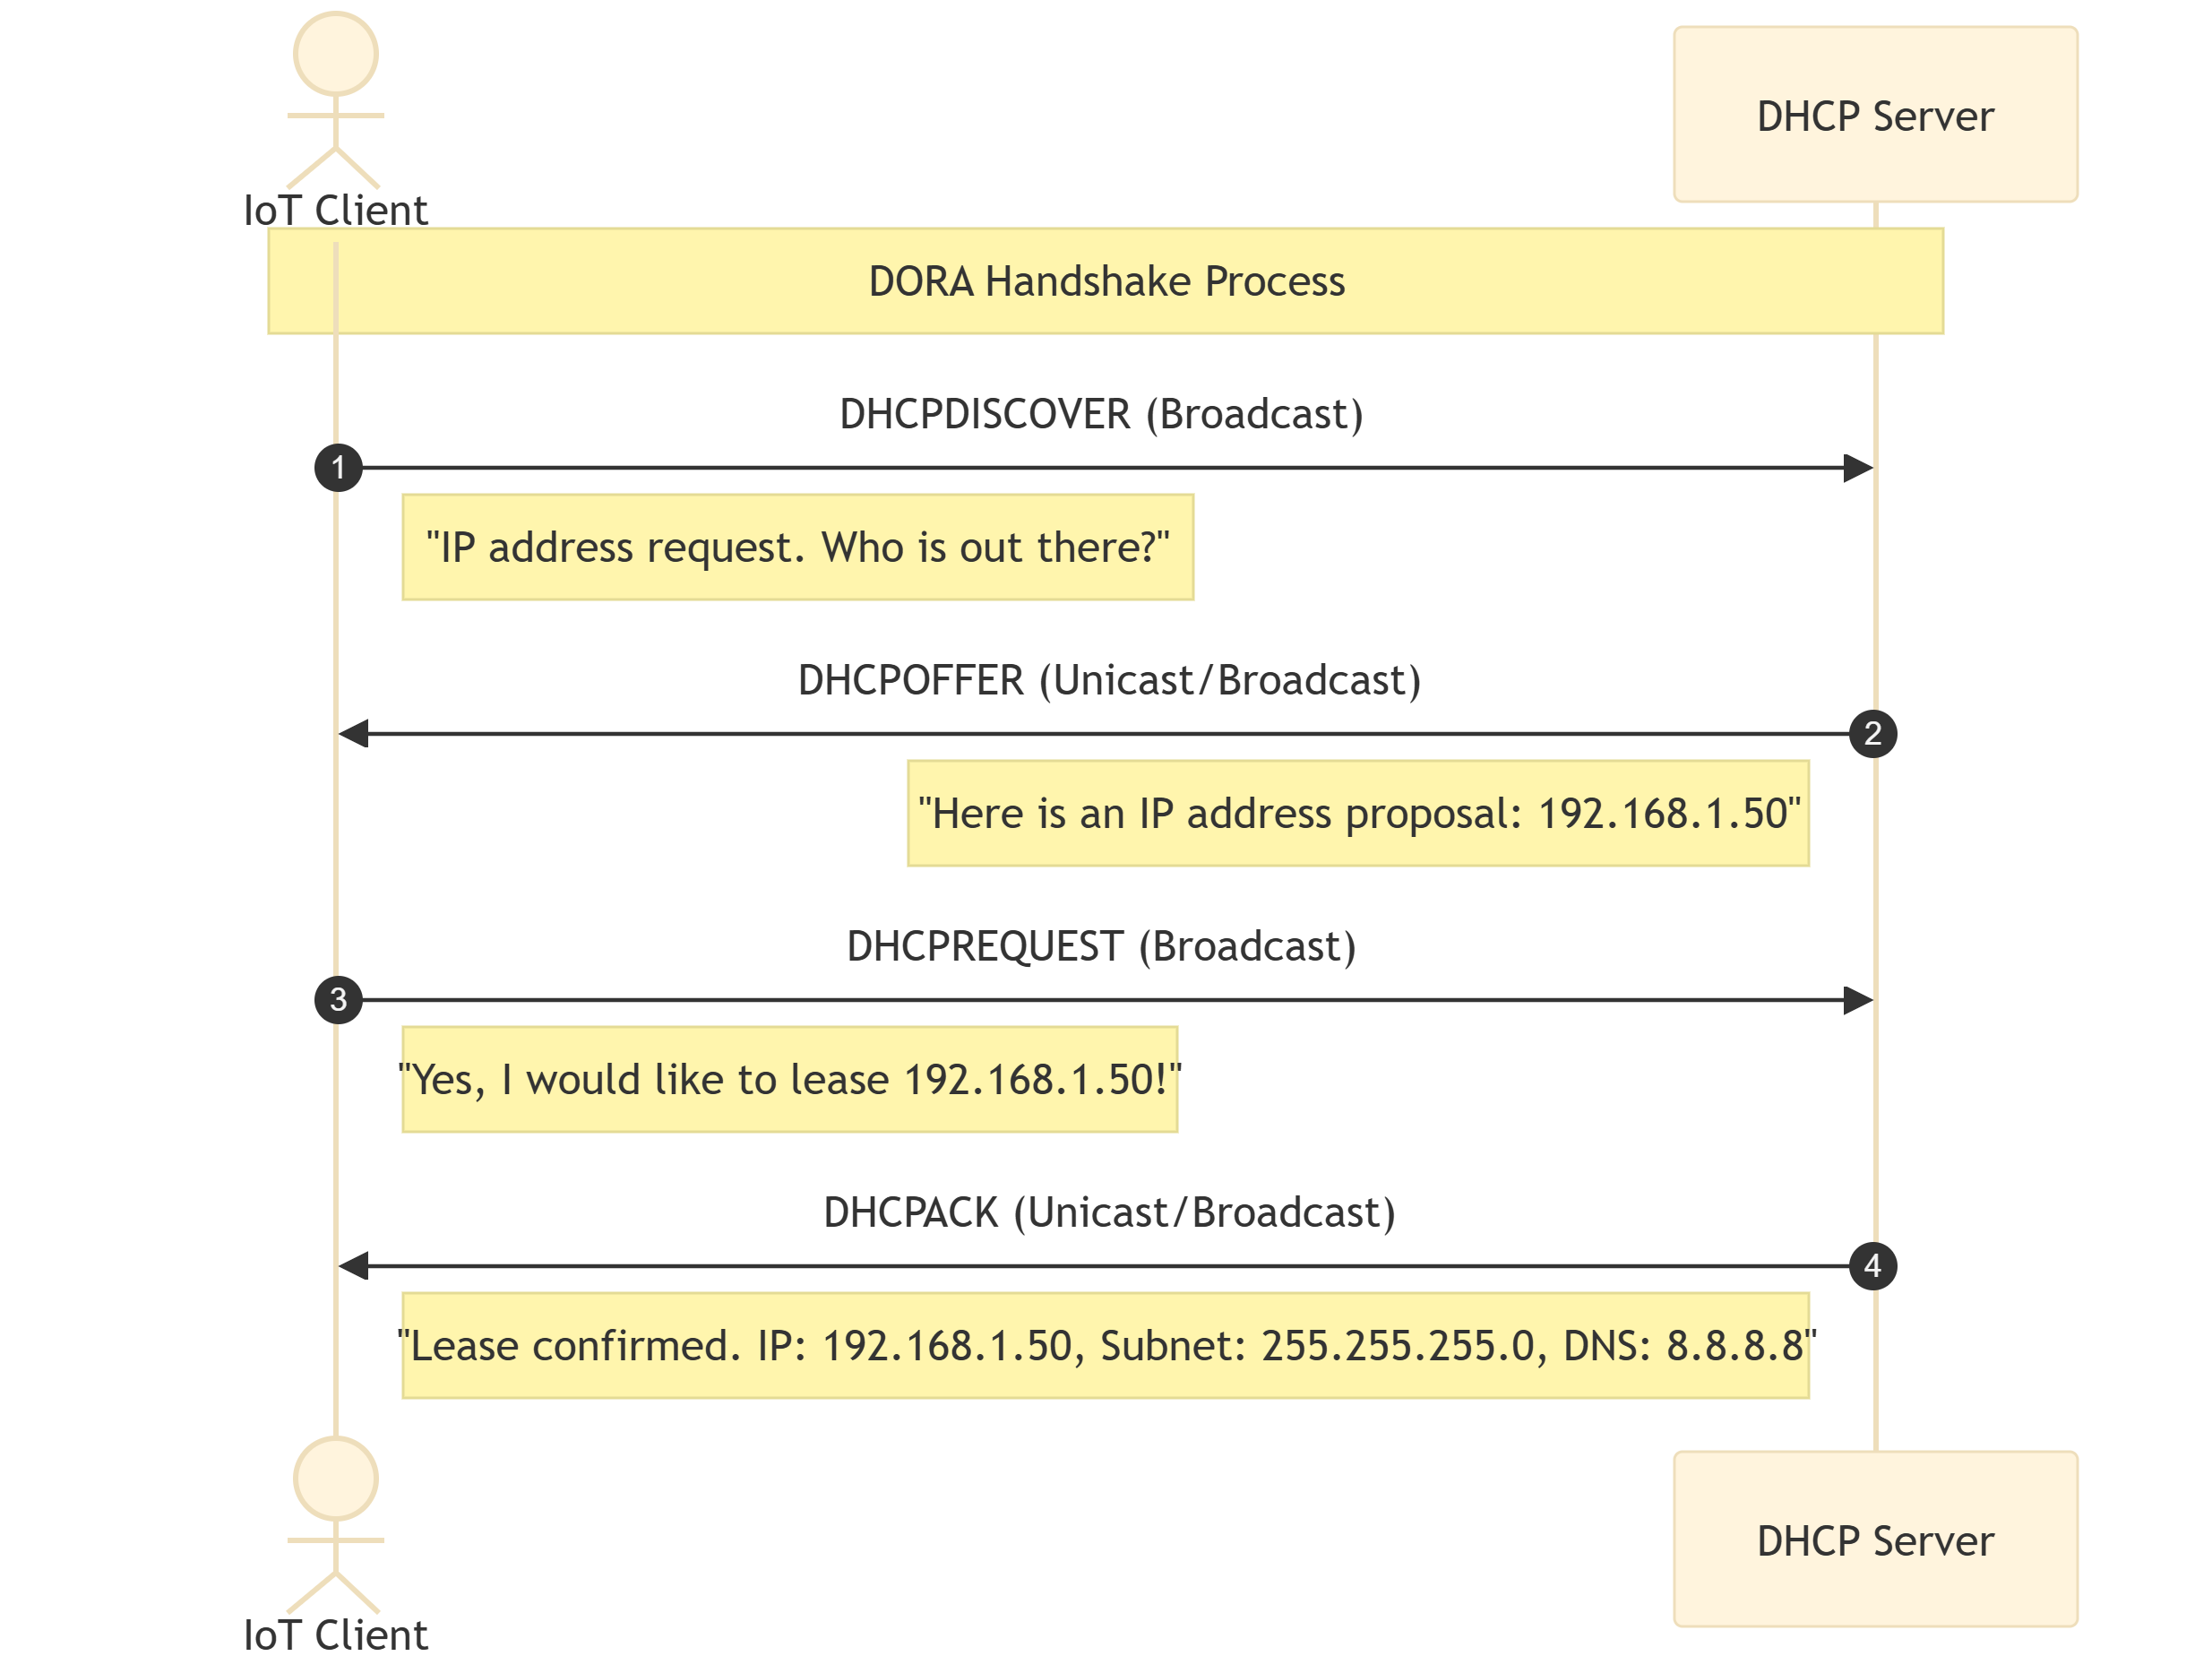
\includegraphics[width=0.75\textwidth,height=0.32\textheight,keepaspectratio]{../Images/chapter_03/dhcp_handshake.png}
\caption{DHCP DORA Handshake}
\end{figure}

\subsection{4. TCP 3-Way Handshake vs. UDP Transmission (Unit III)}
Comparison of connection setup phases.  
\begin{figure}[H]
\centering
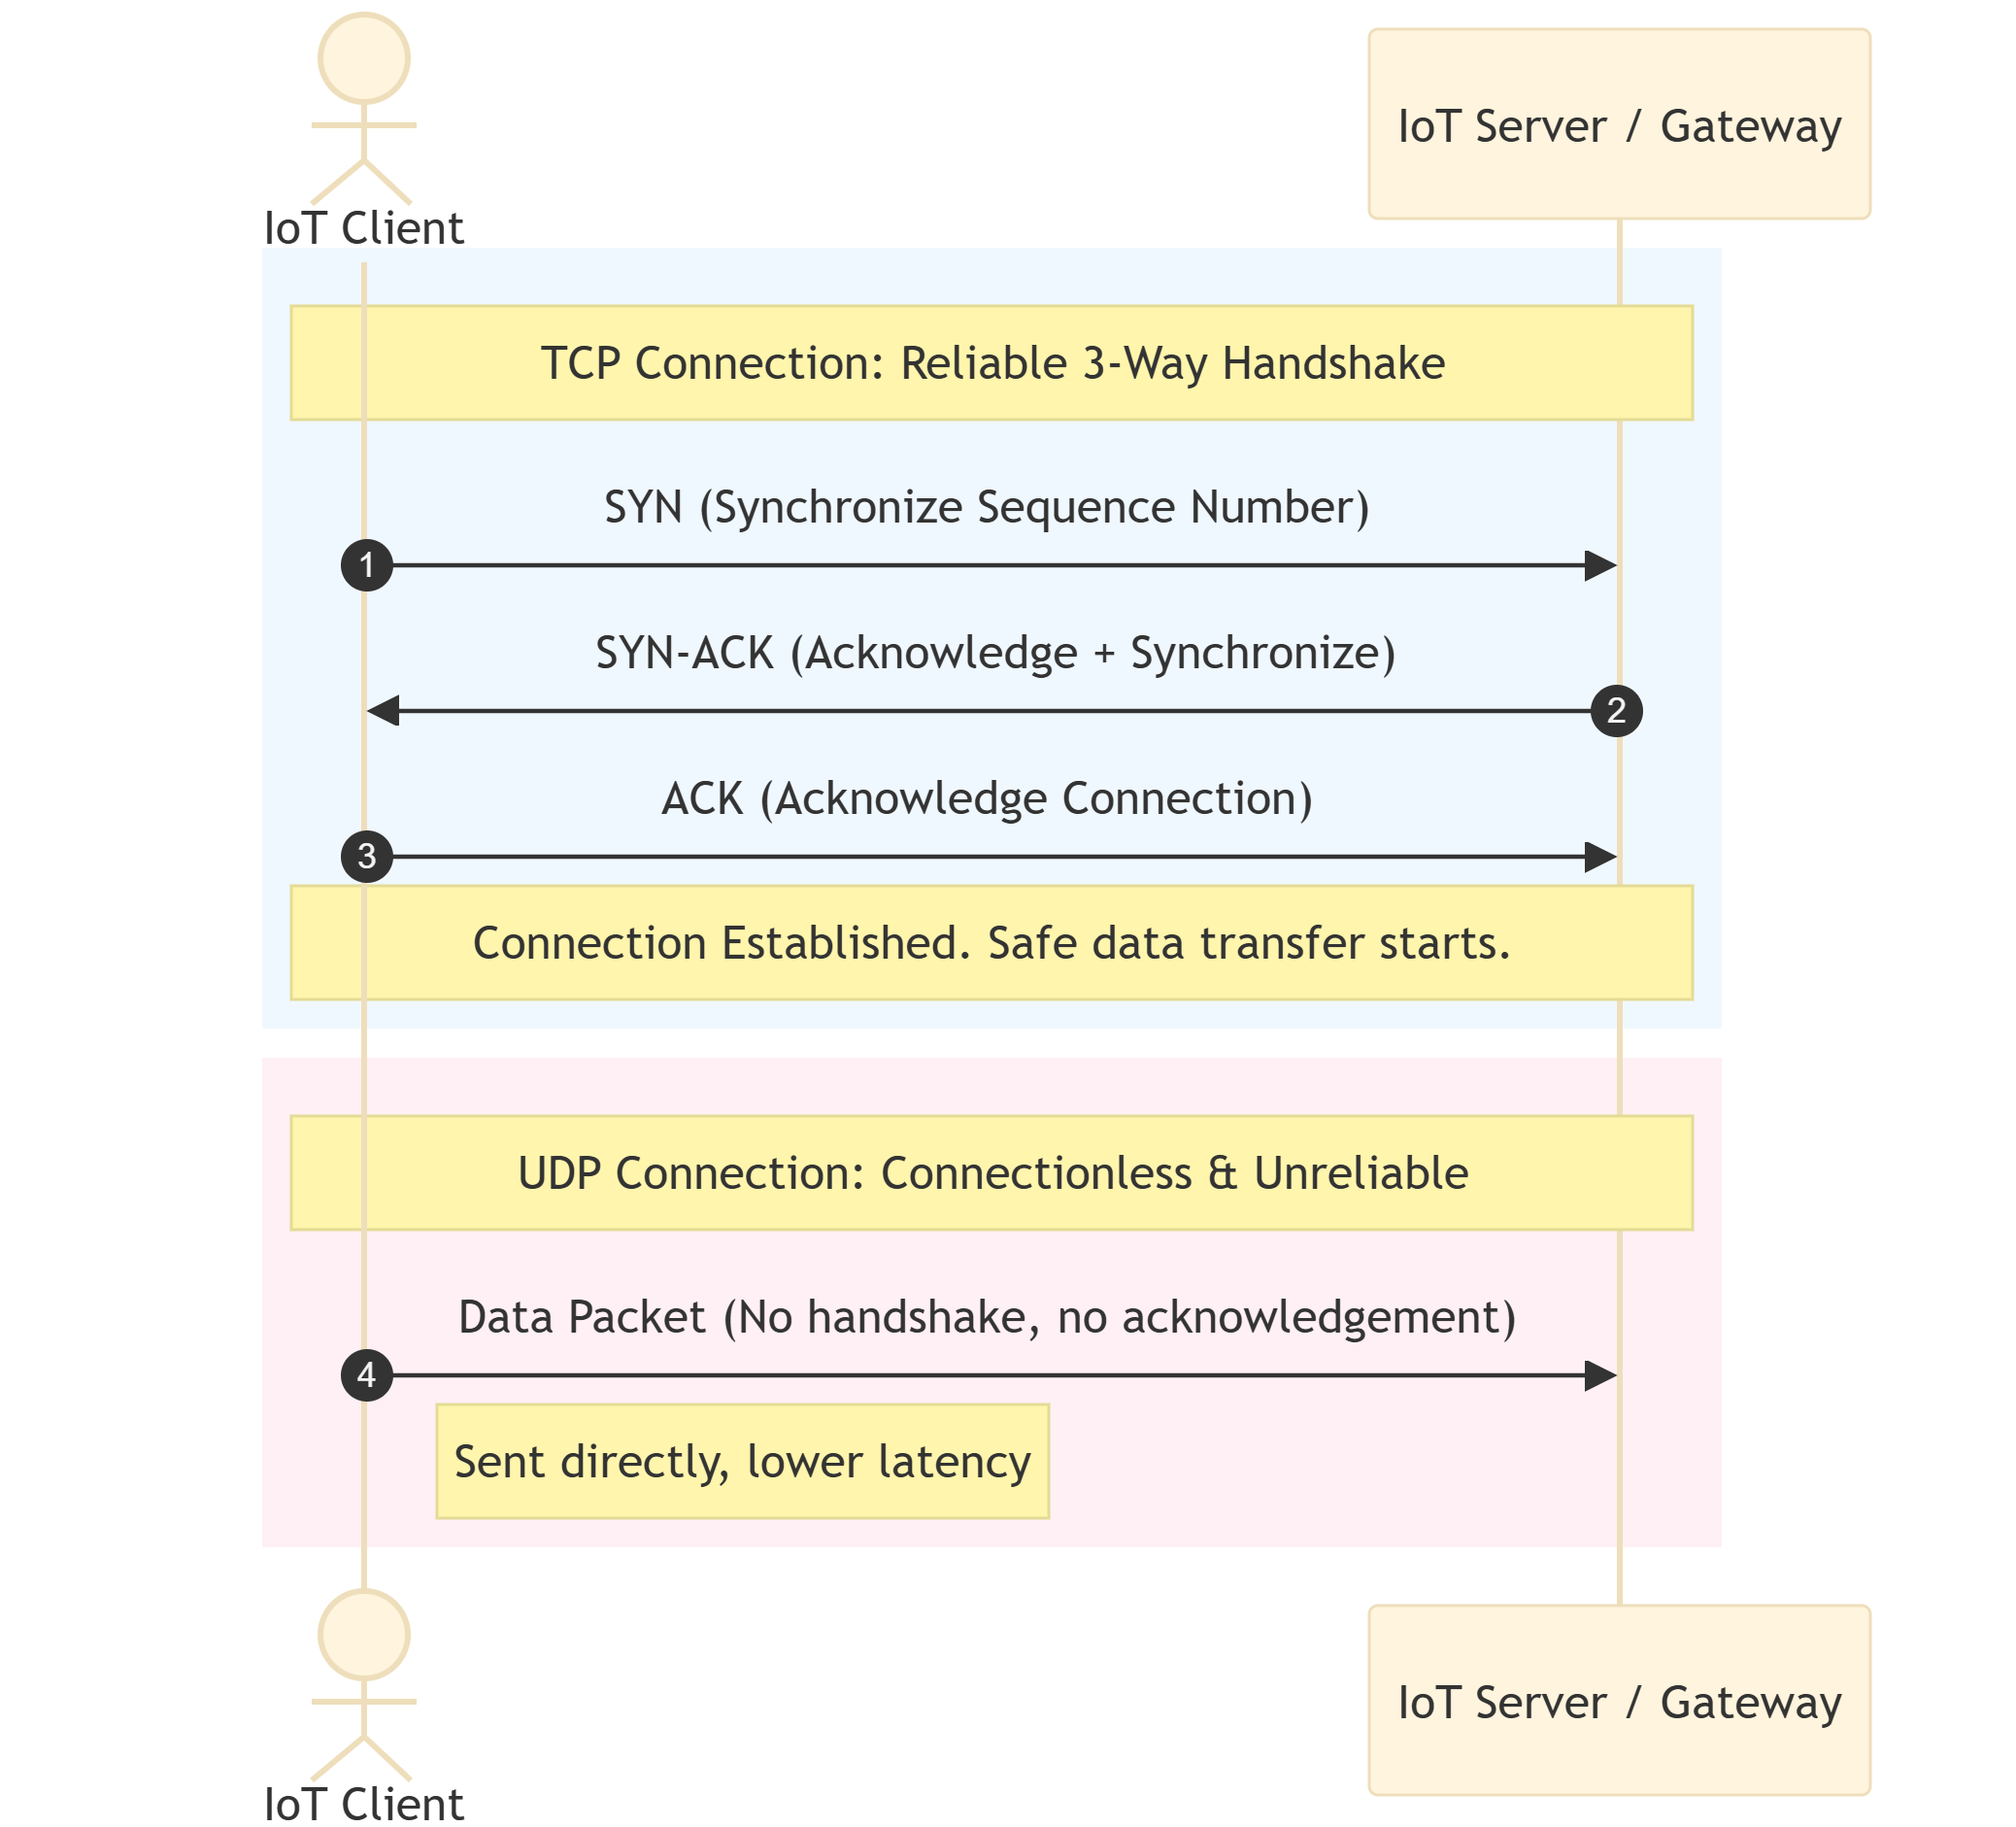
\includegraphics[width=0.75\textwidth,height=0.32\textheight,keepaspectratio]{../Images/chapter_03/tcp_vs_udp.png}
\caption{TCP vs. UDP Protocol Transmission}
\end{figure}

\subsection{5. MQTT Pub/Sub vs. CoAP Architecture (Unit III)}
Broker-driven topics vs. restful client-server calls.  
\begin{figure}[H]
\centering
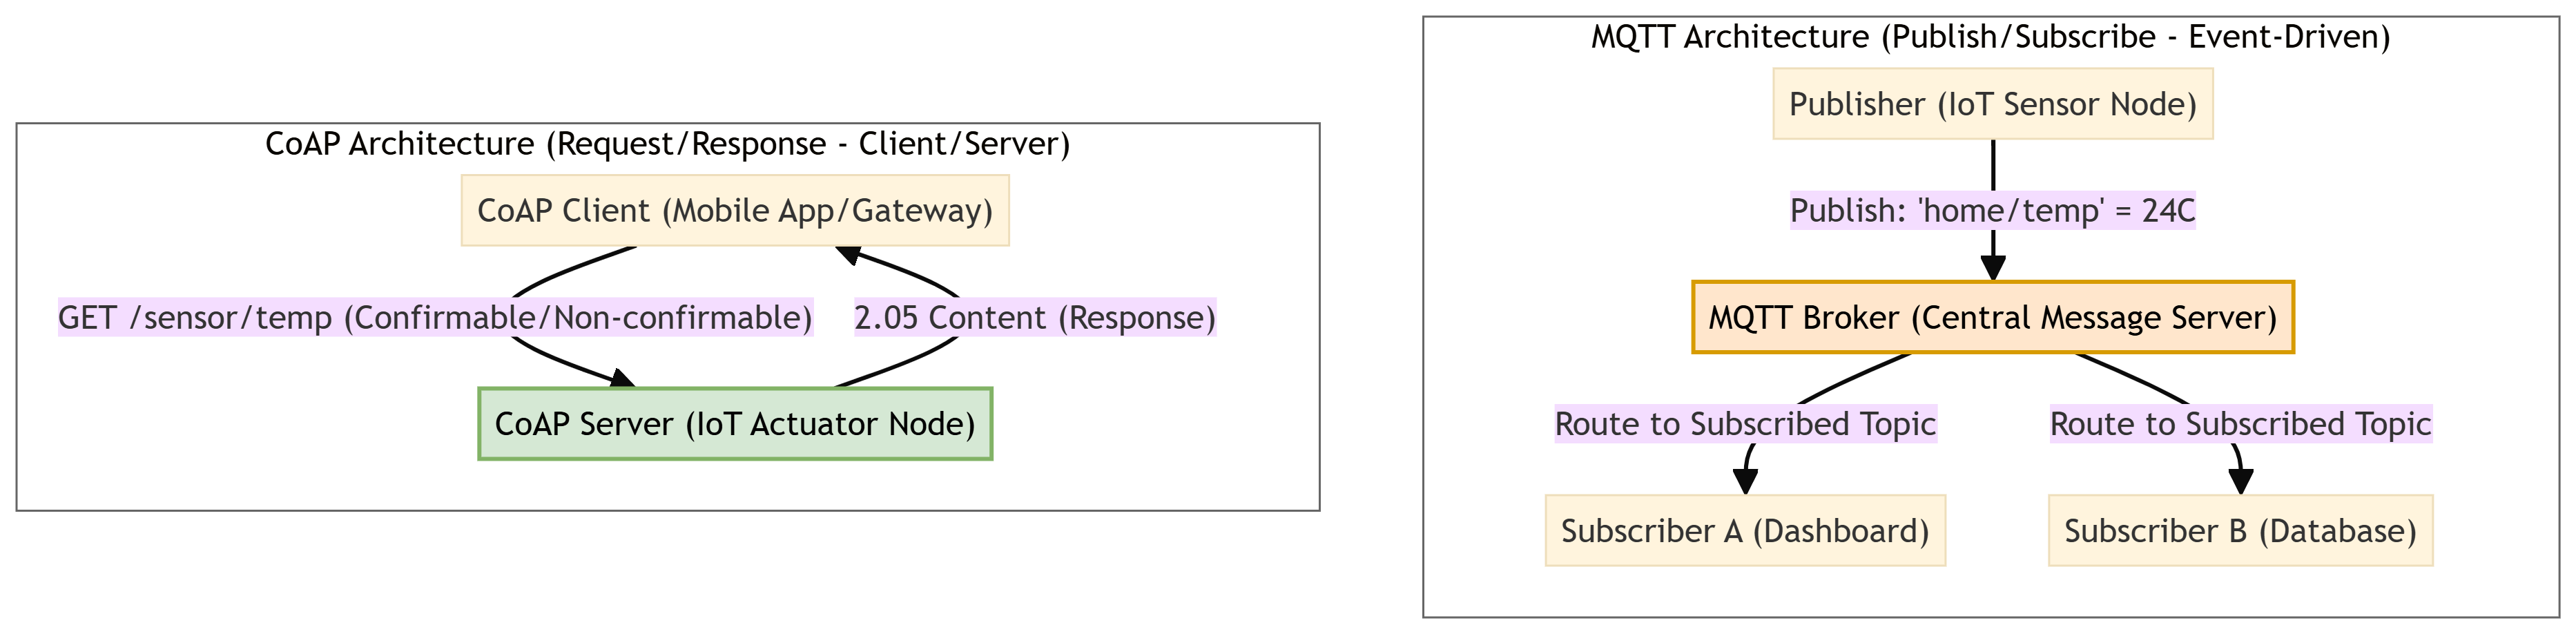
\includegraphics[width=0.75\textwidth,height=0.32\textheight,keepaspectratio]{../Images/chapter_03/mqtt_vs_coap.png}
\caption{MQTT Pub/Sub vs. CoAP Request/Response Architecture}
\end{figure}

\subsection{6. Prototyping Cost vs. Ease Curve (Unit IV)}
Visualizing cost scaling through prototyping stages.  
\begin{figure}[H]
\centering
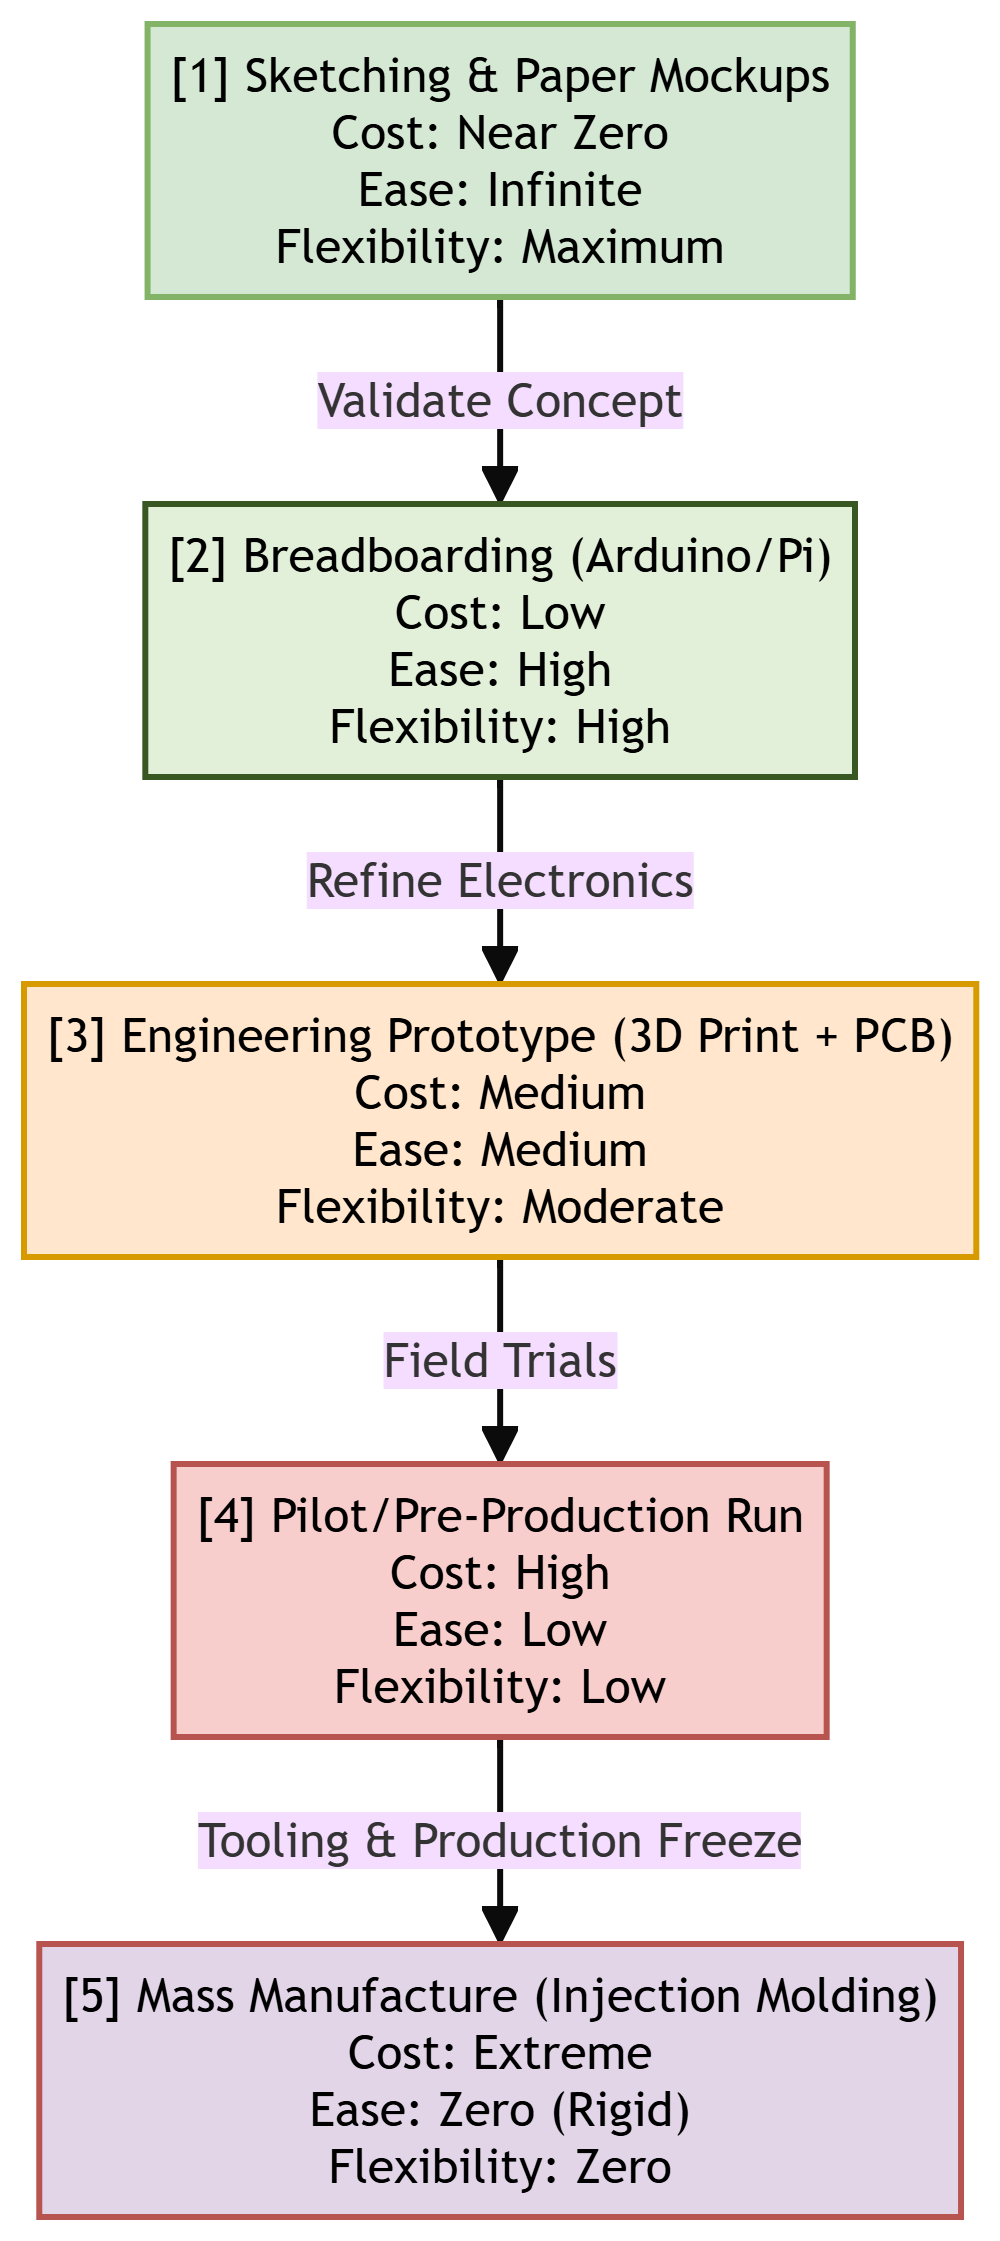
\includegraphics[width=0.75\textwidth,height=0.32\textheight,keepaspectratio]{../Images/chapter_04/cost_vs_ease.png}
\caption{Prototyping Cost vs. Ease Curve}
\end{figure}

\subsection{7. Arduino vs. Raspberry Pi (Unit VI)}
Architectural differences of memory, processors, and peripheral registers.  
\begin{figure}[H]
\centering
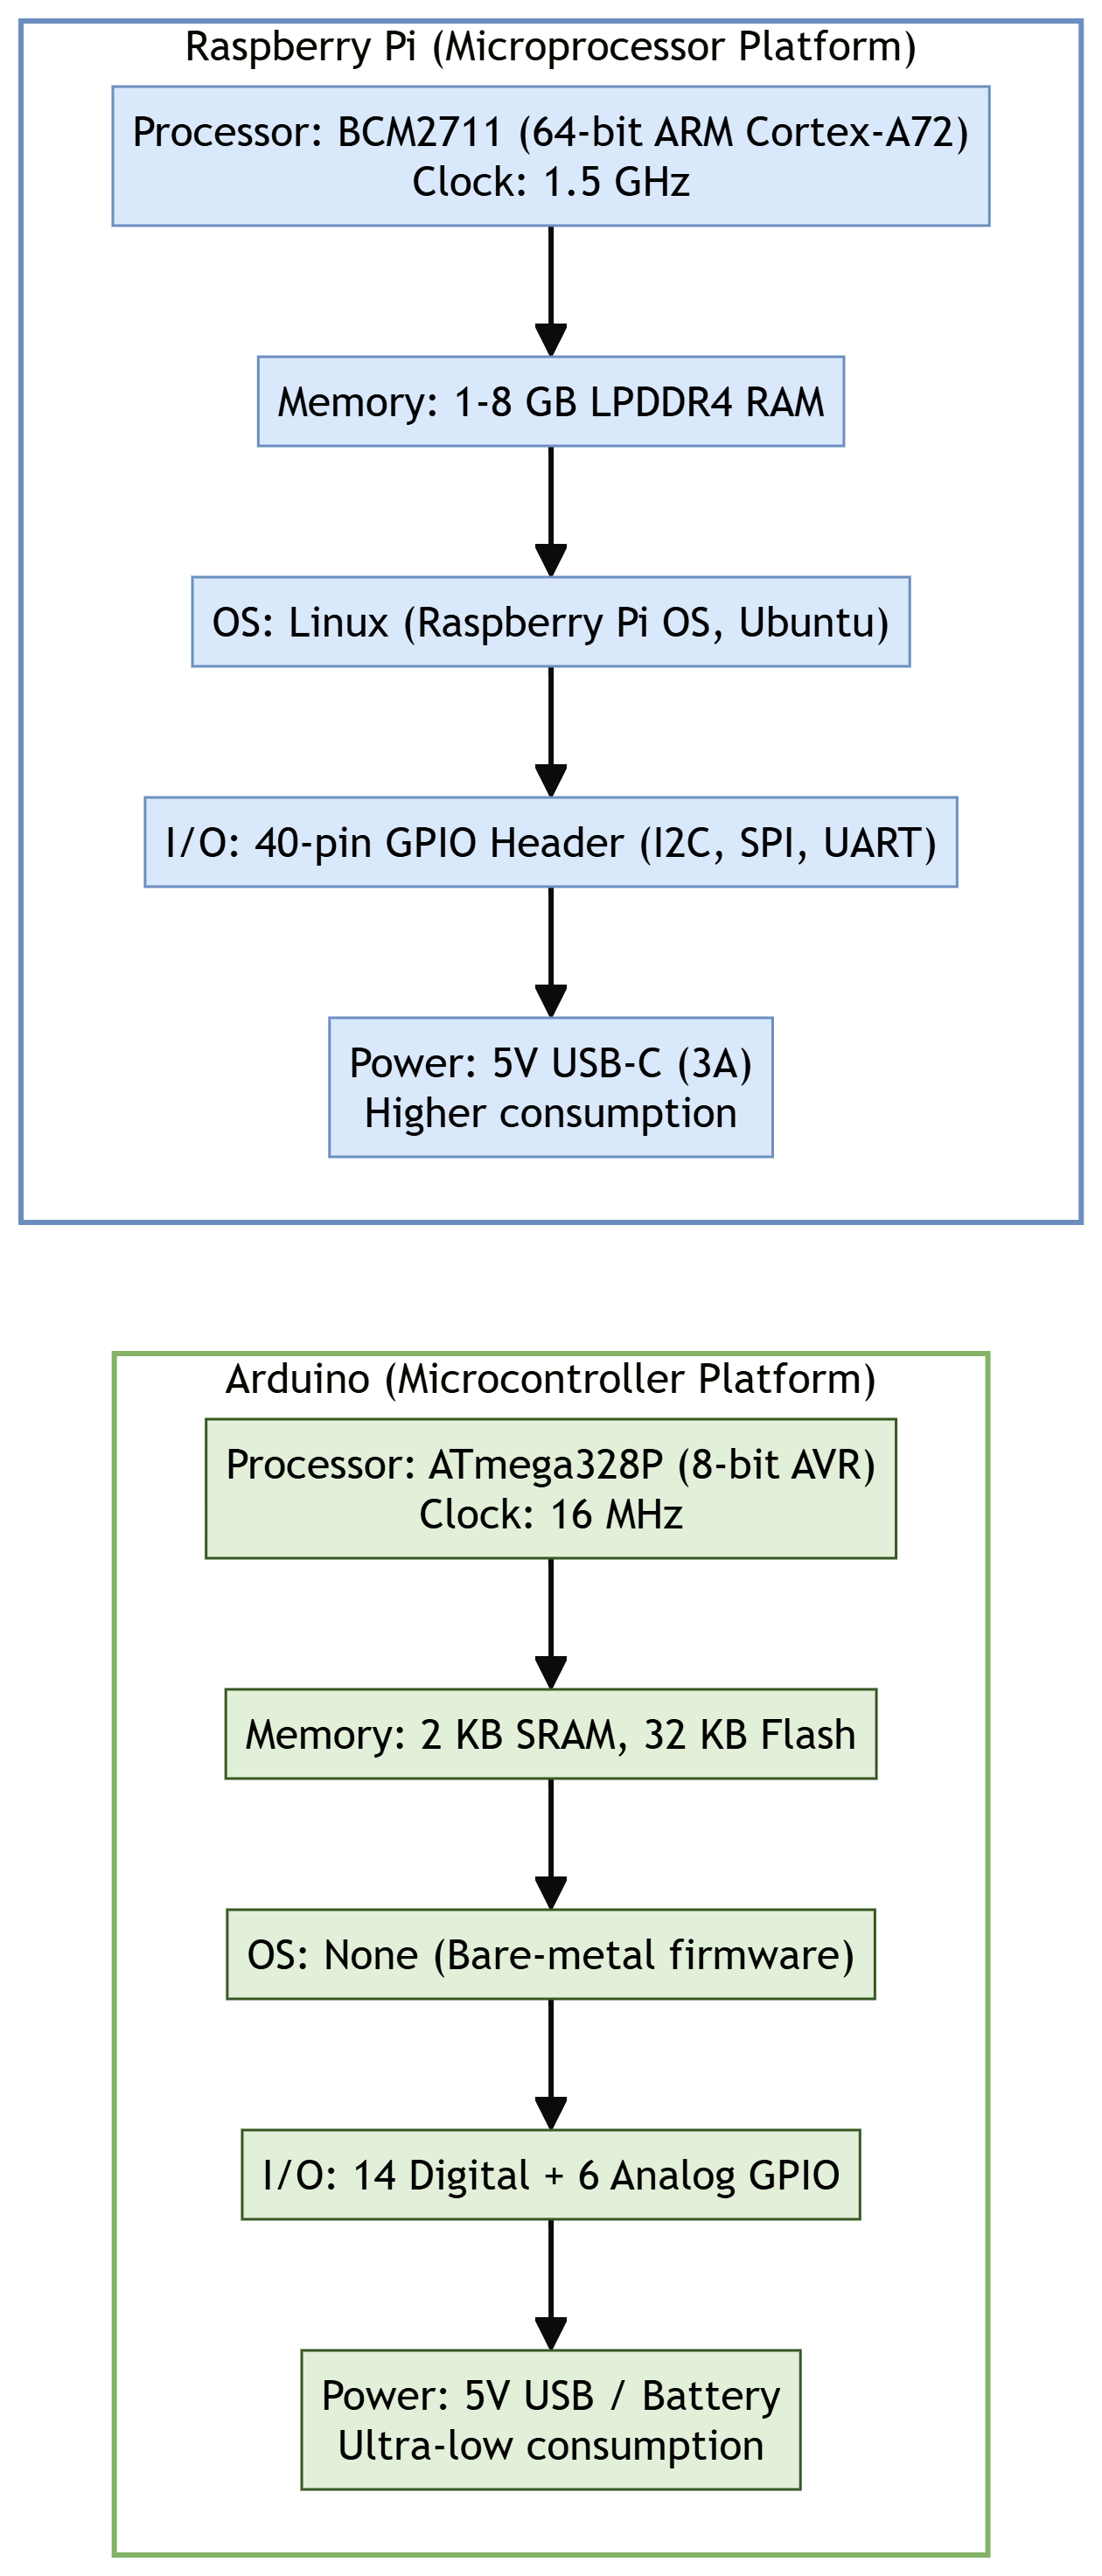
\includegraphics[width=0.75\textwidth,height=0.32\textheight,keepaspectratio]{../Images/chapter_06/arduino_vs_raspberry_pi.png}
\caption{Arduino vs. Raspberry Pi Architecture}
\end{figure}

\subsection{8. Cloud IoT Platform Architecture (Unit VII)}
Multi-layer pipelines (Device $\to$ Gateway $\to$ Processing $\to$ UI).  
\begin{figure}[H]
\centering
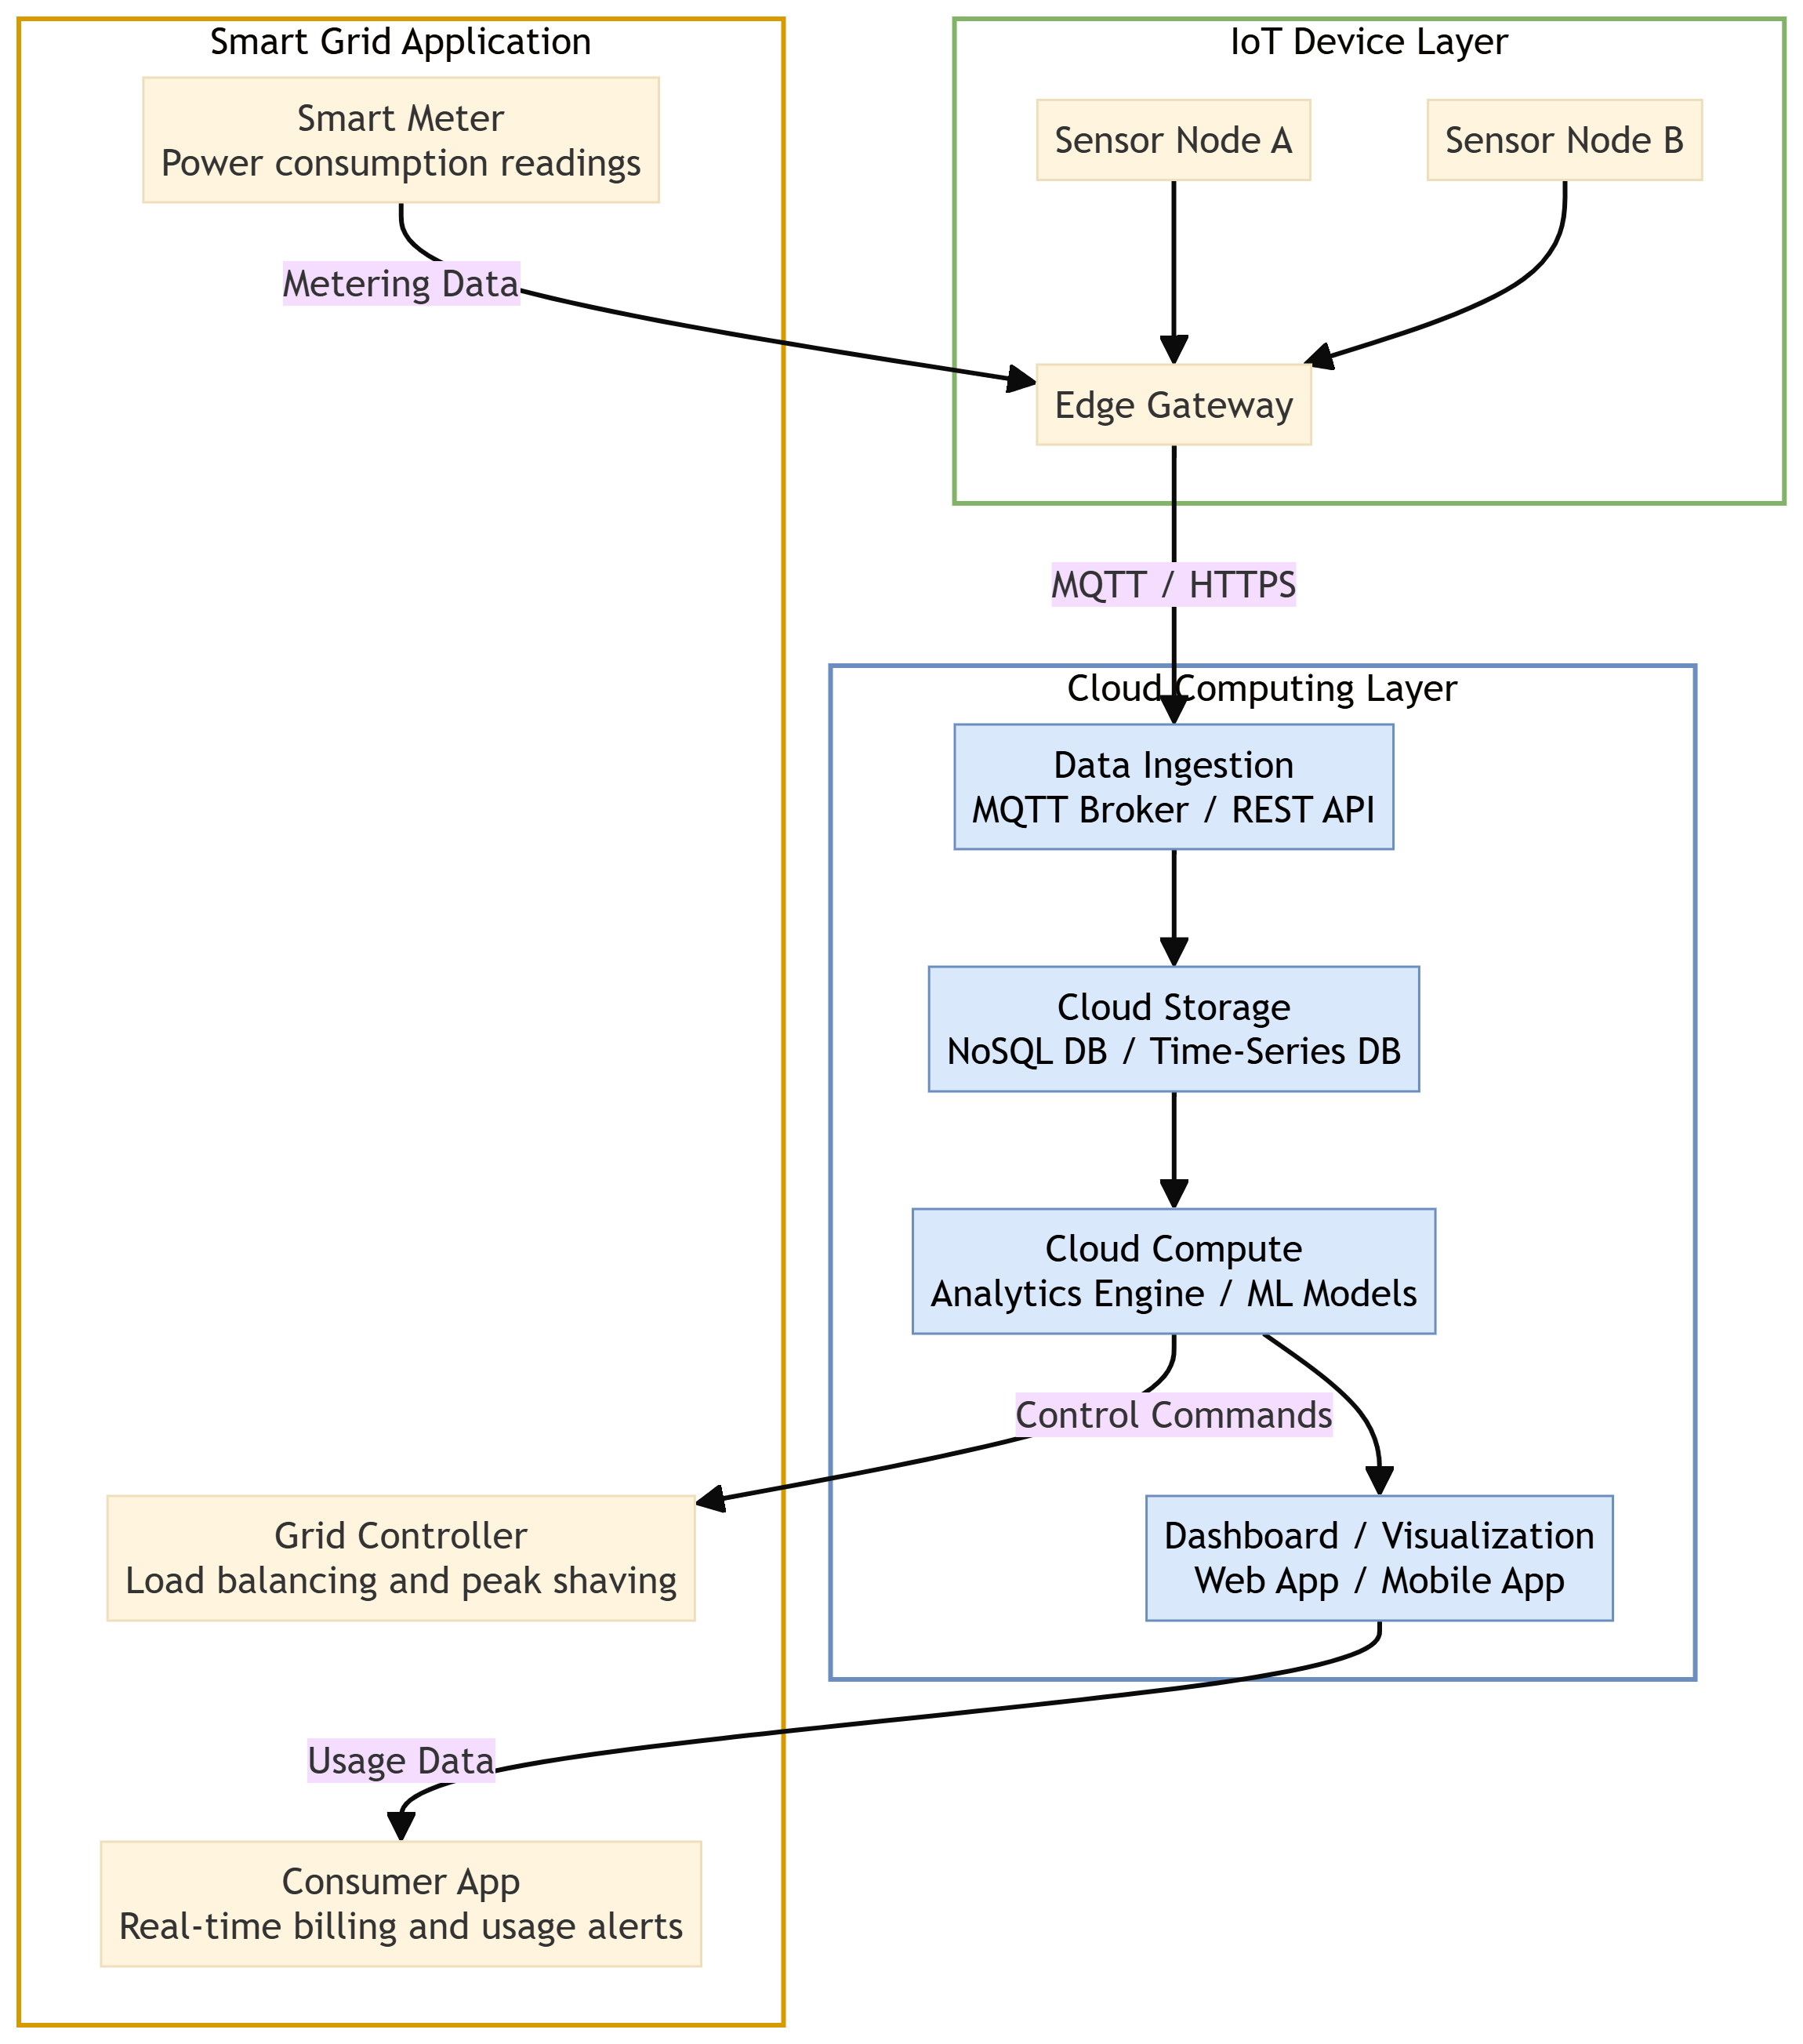
\includegraphics[width=0.75\textwidth,height=0.32\textheight,keepaspectratio]{../Images/chapter_07/cloud_iot_architecture.png}
\caption{Cloud IoT Architecture with Smart Grid Application}
\end{figure}

\subsection{9. PCB Design-to-Manufacture Pipeline (Unit IX)}
Sequence from schematic capture to PCBA functional testing.  
\begin{figure}[H]
\centering
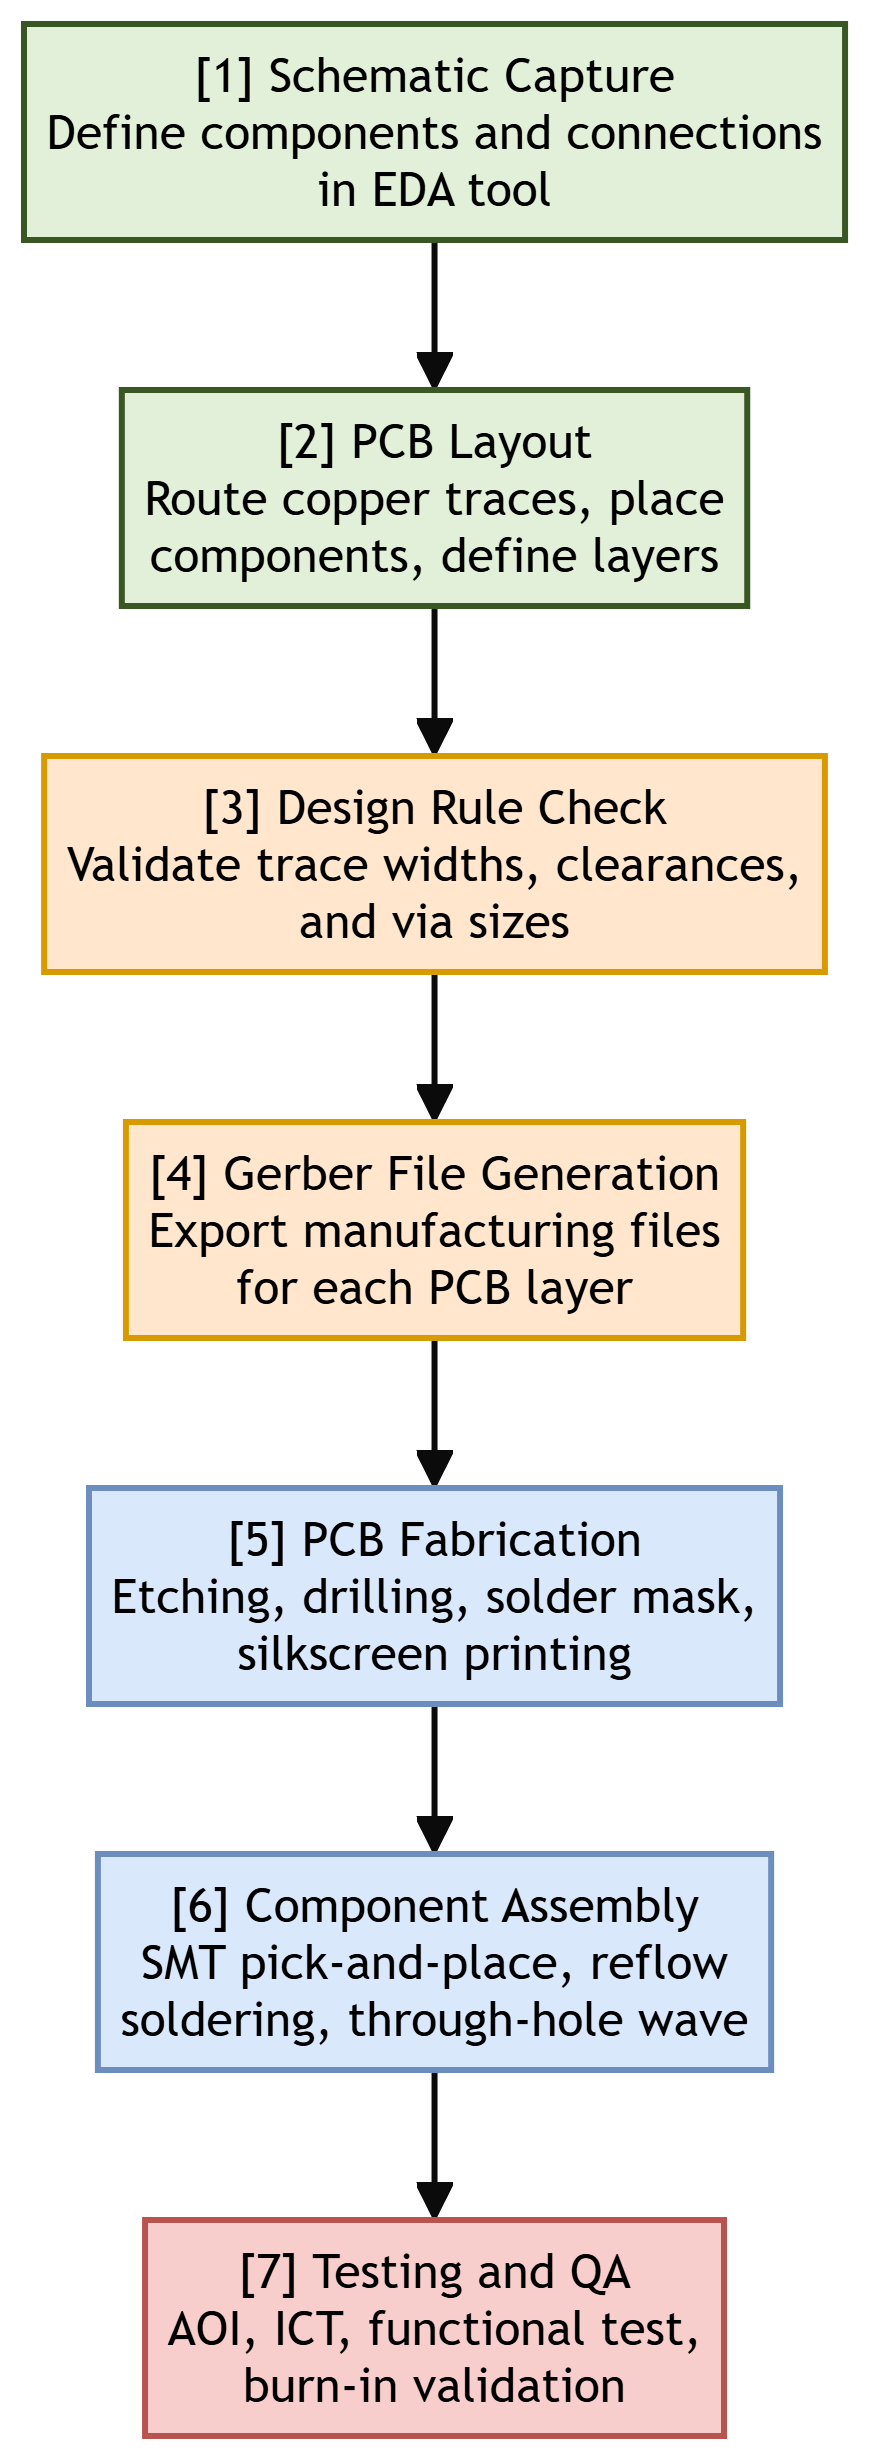
\includegraphics[width=0.75\textwidth,height=0.32\textheight,keepaspectratio]{../Images/chapter_09/pcb_manufacturing_pipeline.png}
\caption{PCB Design to Mass Manufacturing Pipeline}
\end{figure}

\subsection{10. Ethical Challenges of IoT \& Solutions (Unit X)}
Roadmap connecting privacy/control/security threats to engineering mitigations.  
\begin{figure}[H]
\centering
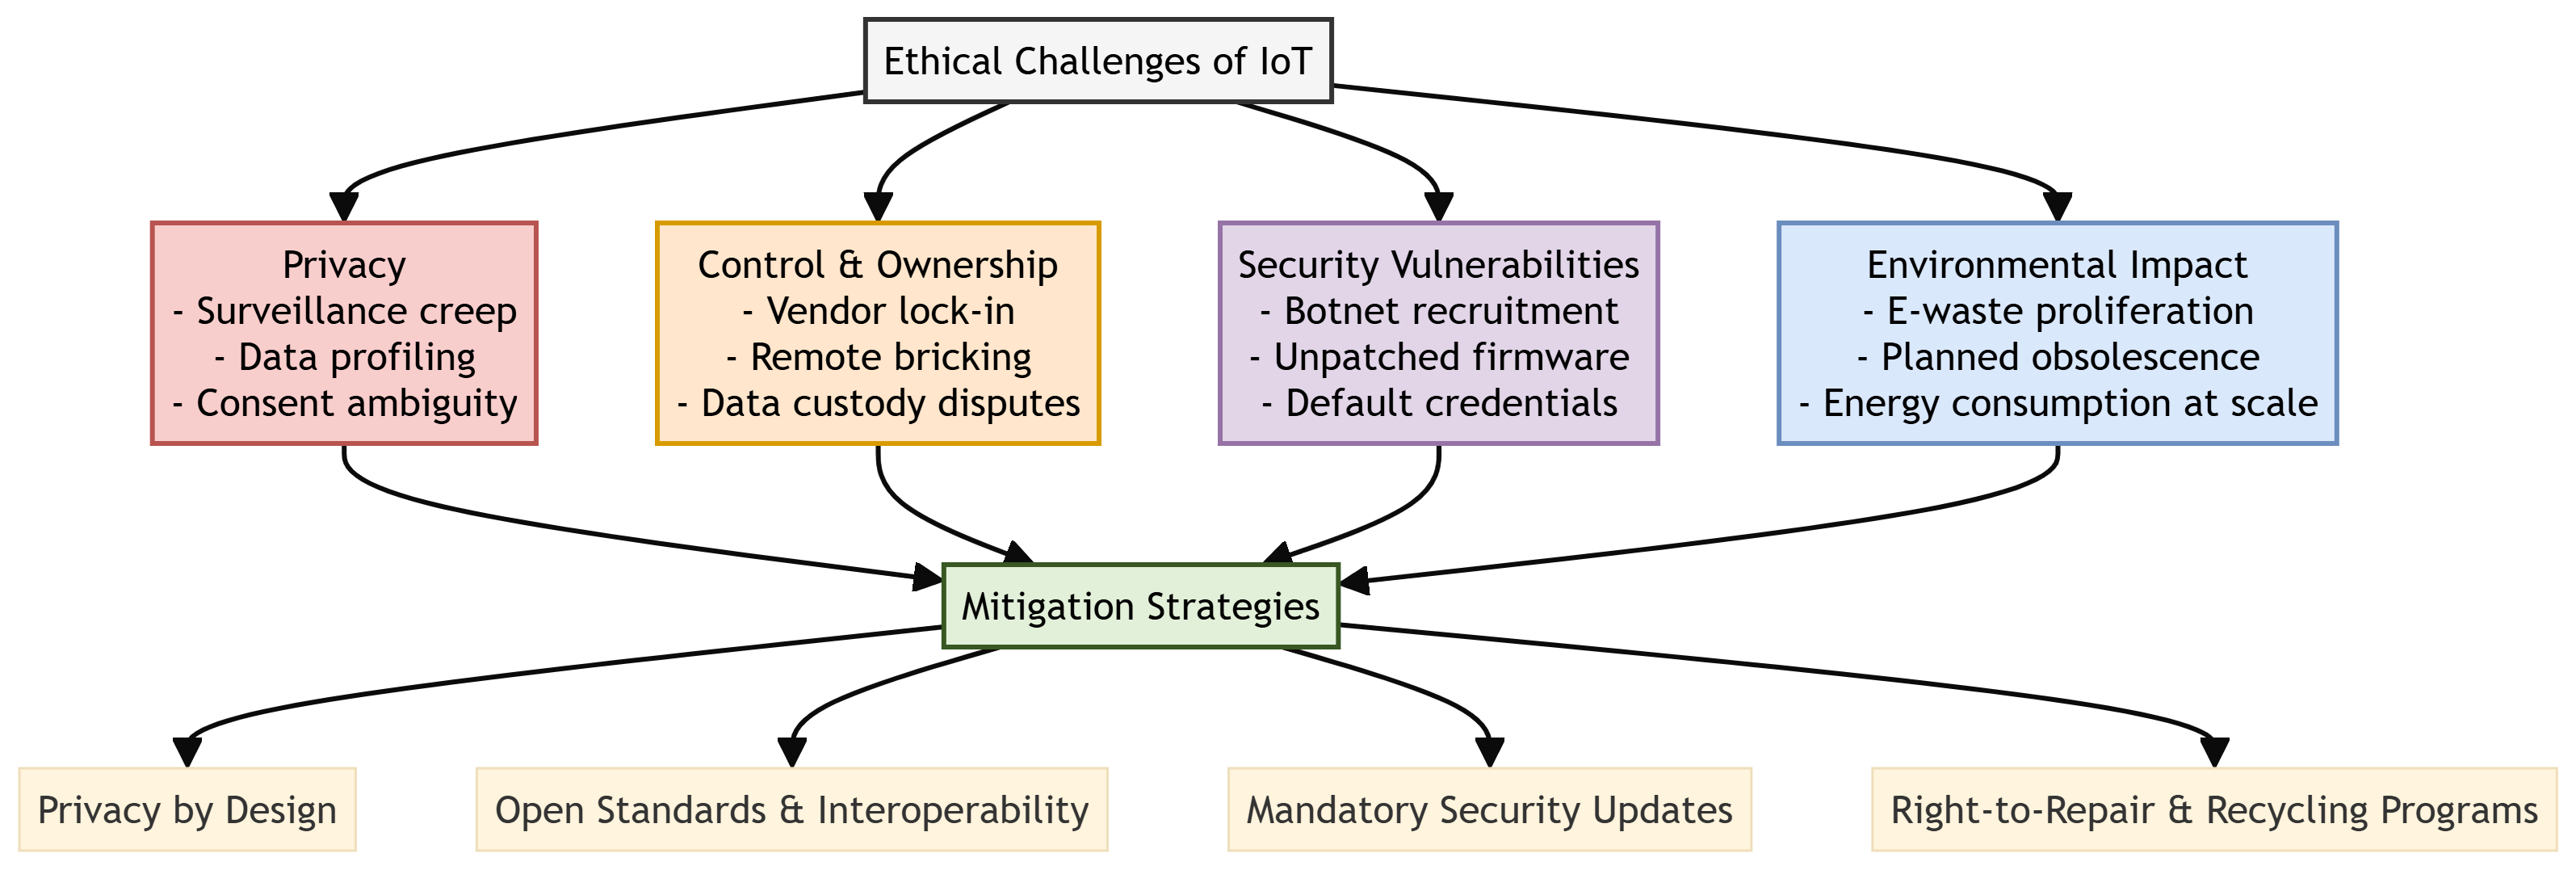
\includegraphics[width=0.75\textwidth,height=0.32\textheight,keepaspectratio]{../Images/chapter_10/iot_ethical_challenges.png}
\caption{Ethical Challenges of IoT and Mitigation}
\end{figure}


\section{Frequently Asked Questions}

\subsection{Q1. Compare Calm and Ambient technologies. [5M]}
\begin{itemize}
  \item   \textbf{Calm Technology:} Technology that informs users without taking over their primary attention (e.g., light patterns, simple sounds). It sits in the peripheral vision and shifts to the center of attention only when needed.
  \item   \textbf{Ambient Devices:} A physical subset of Calm technology designed to show background data changes dynamically (e.g., an Ambient Umbrella that glows blue when rain is forecast).
\end{itemize}

\subsection{Q2. Explain the DORA handshake in DHCP. [5M]}
\begin{itemize}
  \item   \textbf{Discover (Broadcast):} The client broadcasts a request looking for a DHCP server.
  \item   \textbf{Offer (Unicast/Broadcast):} Servers respond proposing an IP address and configuration.
  \item   \textbf{Request (Broadcast):} The client accepts one specific offer and notifies other servers.
  \item   \textbf{Acknowledge (Unicast/Broadcast):} The chosen server confirms the lease and delivers IP settings.
\end{itemize}

\subsection{Q3. Highlight key differences between I2C, SPI, and UART. [5M]}
\begin{itemize}
  \item   \textbf{UART:} Asynchronous, 2-wire, point-to-point communication. Uses start/stop bits instead of a clock pin.
  \item   \textbf{I2C:} Synchronous, 2-wire, multi-master/multi-slave bus. Slower speeds but requires only two pins (SDA/SCL) with addressing.
  \item   \textbf{SPI:} Synchronous, 4-wire, single-master/multi-slave bus. Fastest speeds, uses dedicated Select pins (CS), and operates in full-duplex.
\end{itemize}

\subsection{Q4. Compare HTTP, CoAP, and MQTT protocols. [10M]}
\begin{itemize}
  \item   \textbf{HTTP:} Request-response, TCP-based, verbose text headers. Heavy overhead; unsuitable for constrained nodes.
  \item   \textbf{CoAP:} Request-response, UDP-based, binary headers. Supports REST architecture and Observation mode on constrained microcontrollers.
  \item   \textbf{MQTT:} Publish-subscribe, TCP-based, binary headers (min 2 bytes). Uses a central Broker; event-driven with 3 QoS levels.
\end{itemize}

\subsection{Q5. What testing must be performed on an IoT product prior to mass manufacturing? [15M]}
\begin{itemize}
  \item   \textbf{Hardware:} ESD testing, thermal cycling, drop/vibration testing, and EMI/EMC emissions compliance.
  \item   \textbf{Software:} Unit tests on code blocks, regression tests, and OTA firmware rollback stability tests.
  \item   \textbf{Connectivity:} Wi-Fi range/throughput tests, BLE connection trials, and MQTT QoS delivery confirmation.
  \item   \textbf{Security:} Penetration testing, firmware binary decompilation checks, and secure boot cryptographic validation.
  \item   \textbf{UAT:} Consumer out-of-box experience evaluations and field trials.
\end{itemize}


\section{One-Line Revision Bullets}

\begin{itemize}
  \item   \textbf{Unit I:} IoT is machine-centric (M2M); Enchanted Objects are everyday tools augmented with low-profile smart features.
  \item   \textbf{Unit II:} Design for the periphery (Calm technology); map actions to physical affordances; use metaphors like magic to simplify interfaces.
  \item   \textbf{Unit III:} IPv4 CIDR calculates hosts as $2^{32-N}-2$; DHCP uses the DORA sequence; MAC address is a 48-bit burned-in physical ID.
  \item   \textbf{Unit IV:} Prototype incrementally to keep costs low; use open hardware to speed up development via existing libraries and forums.
  \item   \textbf{Unit V:} 3D printing is additive but slow; laser cutting is 2.5D and fast; CNC milling carves 3D shapes from metal/wood with tight tolerances.
  \item   \textbf{Unit VI:} MCUs run bare-metal loops; MPUs require operating systems; keep the antenna case clearance at least $10\text{ mm}$ to prevent detuning.
  \item   \textbf{Unit VII:} HTTP is synchronous pull; WebSockets are persistent full-duplex TCP tunnels; MQTT is asynchronous broker-driven pub/sub.
  \item   \textbf{Unit VIII:} Write low-power code (use sleep states, avoid floats); scale startups iteratively using the Lean "Build-Measure-Learn" cycle.
  \item   \textbf{Unit IX:} PCB design yields Gerber files; PCBA quality is checked using AOI, ICT, and Burn-In stress chambers; enclosures require high-cost injection molds.
  \item   \textbf{Unit X:} Smart cities use dynamic lighting and ITS to save energy; protect user rights by implementing Privacy by Design and open interfaces.
\end{itemize}
